% This is samplepaper.tex, a sample chapter demonstrating the
% LLNCS macro package for Springer Computer Science proceedings;
% Version 2.20 of 2017/10/04
%
\documentclass[runningheads]{llncs}
%
\usepackage{graphicx}
\usepackage{amsmath}
\usepackage{amssymb}
% Used for displaying a sample figure. If possible, figure files should
% be included in EPS format.
%
% If you use the hyperref package, please uncomment the following line
% to display URLs in blue roman font according to Springer's eBook style:
% \renewcommand\UrlFont{\color{blue}\rmfamily}

\begin{document}
%
\title{Wide exploration with smooth action}
%
%\titlerunning{Abbreviated paper title}
% If the paper title is too long for the running head, you can set
% an abbreviated paper title here
%
\author{Emmanuel Daucé\inst{1}\orcidID{0000-0001-6596-8168}}
%
\authorrunning{E. Daucé}
% First names are abbreviated in the running head.
% If there are more than two authors, 'et al.' is used.
%
\institute{Institut de Neurosciences de la Timone, CNRS/Aix-Marseille Univ, France
\email{emmanuel.dauce@univ-amu.fr}}
%
\maketitle              % typeset the header of the contribution
%
\begin{abstract}
%The abstract should briefly summarize the contents of the paper in
%150--250 words.

\keywords{First keyword  \and Second keyword \and Another keyword.}
\end{abstract}
%
%
%
\section{Introduction}

Recent developments in artificial intelligence have produced important qualitative leaps in the field of pattern recognition (identification of objects, faces, speech recognition, ...) in video games and assisted driving. 
They have also enabled the emergence of generative models for images, video and language. The key element that explains the success of these algorithms is the extraction of statistical invariants from data, via auto-encoding mechanisms, from data sets of arbitrary dimensions. The codes are constructed during training using the gradient descent technique. After learning, they provide synthetic descriptors of the situations encountered, which are necessary and sufficient for the production of appropriate responses.  Once learned, they thus constitute very powerful generative models of the input data. Nevertheless, the learning of these invariants currently requires a considerable amount of data, real or simulated, which makes the learning algorithms dependent on the available databases, and gives the data collection (or simulation) process a disproportionate place. Furthermore, while the capabilities of these algorithms approach (and sometimes exceed) those of human subjects for specific tasks, they never achieve the universal skills and general adaptability of the human brain. 

Nevertheless, a number of tasks considered as simple, falling under universal competences specific to the animal world, are struggling to find a convincing artificial implementation... This is the field of action selection and motor control. For instance, a number of tasks involving the fine manipulation of objects, as well as movement in natural environments, and their combination through motor commands updated in real time according to the state of the sensors, are major challenges that are currently concentrating the efforts of the main players in the digital revolution.
Reinforcement Learning in particular remains rather limited in the field of robotic control (compared to video games). The huge developments obtained on virtual environments (from nothing) are difficult to transfer to real robotics (millions of parts/millions of tests, risk of breakage...) and simulators are expensive to develop.

The brain, on the other hand, is capable of developing motor skills in a very wide range of areas over a long developmental phase.   
The main function of the brain is to enable movement, to orientate the body and to enable it to use the environment to its own advantage. The control of an articulated body is particularly complex, and if we consider humans, it takes about a year to learn bipedal walking. The brain's ability to learn new abilities and skills is particularly striking, but it is not specific to humans. The brain in general adapts to its environment. Animals modify their behaviour flexibly according to their own history. 

The nervous system is characterized by a high degree of noise and variability: synapses are stochastic, neurons are fatiguable, synaptic connections are plastic. Neurons taken at the individual level are extremely unreliable as a unit of information processing (to the same extent as would be biologically possible). There is an "excess" of noise in the nervous system, which leads to (i) an ability to "produce" noise/information; (ii) an ability to "sample" the response space; (iii) a principle of scan/exploration/collection (foraging) of the sensory/motor space (one does not immediately return to where one has already explored).

Physiology
\begin{itemize}
	\item >80\% reciprocal connections in the cortex (Van Essen et al, 1992)
	\item Intrinsic Activity (Fox et al, 2006)
	\item Stochastic Behaviour (Shadlen, Newsome, 1998)
	\item Plasticity of Hebb (Bi and Poo, 1998)	
\end{itemize}
Motor control
\begin{itemize}
	\item end-effector control  (independent of the starting point) (Graziano et al, 2002)
	\item Spatial and temporal compositionality of motor tasks (Diedrichsen \& Kornysheva, 2015, Kadmon Harpaz et al, 2019)
\end{itemize}


The probabilistic view to learning cause-effect relationships is at the core of many recent developments in machine learning, with a body of optimization techniques known as “variational inference” implementing model training from data [1]. One key idea is here to take inspiration from some theories developed in machine learning to reconsider brain modelling at the light of probabilistic inference and optimization.
A first and not  yet fully unveiled example is how the brain learns the consequence of its own action though experiencing interactions with the world [2]. A second example in vision is how the eye selects its next saccade in order to deepen the understanding of its visual environment [3].
Taking motor control learning and action selection as a main guideline, our objective is to decipher the respective contributions of information seeking [4], learning improvement [5] and utility maximization [6] in the selection of actions in an ecological setting, with both perspectives in modelling brain function and developing innovative brain-inspired machine learning techniques for control and robotics.

[1] Kingma, D. P., \& Welling, M. (2013). Auto-encoding variational bayes. arXiv:1312.6114.

[2] Daucé, E. (2016). Predicting the consequence of action in digital control state spaces. arXiv:1609.09681.

[3] Daucé, E, Albigès, P and Perrinet, L (2019) Learning where to look: a foveated visuomotor control model. CNS*2019.

[4] Mohamed, S., \& Rezende, D. J. (2015). Variational information maximisation for intrinsically motivated reinforcement learning. NIPS.

[5] Schmidhuber, J. (1991). Curious model-building control systems. IJCNN.

[6] Sutton, R. S., \& Barto, A. G. (2018). Reinforcement learning: An introduction. MIT press (2nd ed.).

\section{Method}

Formally speaking, the set of circuits, neurons that process the sensory signals and produce a motor response
is the \emph{control space} and the body, muscles and environment is the \emph{operation space}. 
The circuits and neurons are digital
The body and environment is a continuous physical system 

Their are generally two ways to design controllers.  
In analog control, both the controller and the environment are dynamical systems. 
More precisely : a controller is organised around its sensors / actuators with a measure and 
an action. The controller acts on the environment (change according to internal states). 
The environment acts on the controller (that changes according to its internal state -- memory)
The control of a dynamic system generally relies on a \emph{model}. The controller is capable to mimic the
behavior of the environment, and know the effect of its actions on the environment. When a certain objective is given, it can 
act so as to reach the objective through \emph{model inversion}.
This kind of controller needs a model, that is generally given. When no model is given, it needs both to train a model from 
the data, and train an inverse model that fits the action to the objective.
A main drawback of model inversion is the fact that, in most cases of interest (like the control of an articulated body), the models are not invertible and no single definite control can be established from a given objective. 

In contrast, in a digital (discrete) world, all you
need is to establish a one to one correspondence between stimuli and actions. For a given stimulus, you need to find the action by
matching the input with a template action. Given a set of pre-defined actions, all you have to do is just pick the one that matches the most the input.  
In order to learn how to act, the agent is guided by a reward signal (much cheaper than an exact set point).
%much easier to train from data. 
But : the rewards can be sparse.
Utility-based control defines an important quantity : the utility : the long term sum of rewards.
The Reinforcement Learning agent is agnostic about what the world is. It is just acting so as to maximize the utility.
Supported by the solid principles of dynamic programming, this agent is in principle easier to train than an analog one, but
a hidden difficulty lies in finding a good training dataset for the agent. A classical problem in that case is the lack of sampling efficacy due to the closed-loop structure of the control task, where the examples encountered are statistically dependent on the controller parameters, 
providing a risk of a self referential loop and local optimum.

A main difference between the two approaches is thus the presence (or the absence) of a definite model of the external world.   Knowing the effect of our own actions in the world provide ways to anticipate and do planning to reach an objective, at the cost of maintaining and updating a model of the world. 

The opposition between model-free and model-based control has provoked many debates in the reinforcement learning community, with a preference toward model-free approaches for they are cheaper to maintain and easier to control, leaving unsolved the problem of the sampling efficacy and causing very long training sessions in moderately complex environments.
 
Our argument here is that the sampling efficacy is bound to the problem of training a model, and one can not expect to have an efficient sampling without a minimal model of the \emph{effect} of action. This model does not need to be perfectly accurate, but it needs to be good enough to allow the agent to efficiently sample its environment in order to grab all the disposable information in relation to the task at hand. We assert here that a simple \emph{effect model} is enough to provide all the needed variability in the effect of an action or a policy. 

Our approach is different from the `curious'', and ''novelty seeking'' agents.

In order to circumvent this problem, a body of work has developed curiosity and novelty-seeking in agents, independently from the utility of actions.  [REFS]
Novelty seeking relies on building a model of the environment to which the current data is compared. A data showing inconsistencies with the model is considered as "interesting" and should attract the attention of the agent, independently of its extrinsic value.  

We assume for simplicity that the environment is not hidden to the agent, i.e. the environment is fully observable. We also assume a discrete updating of states and actions, like in classic reinforcement learning.
Then, if $s$ is the state of the environment (or a context), and $a$ an action performed by the agent, consider $e$ as the \emph{effect} of the action performed by the agent in that particular state. The effect can be a short-term effect, like reading a new state from the environment. It can also be a long term effect, like winning or loosing a game, or reaching an objective $s*$ in the future. Because there is a lot of uncertainty on the effect of an action, it is modeled as a probability distribution $p(E|s,a)$.
When the effect is not dependent on a context, it can be noted more simply $p(E|a)$.
Given a certain policy $\pi(a|s)$, one can also consider the average distribution of effects obtained when applying that specific policy, namely $p(E|s) = \mathbb{E}_{a\sim \pi(A|s)} p(E|s,a)$.  

In goal-directed control, if $e$ is an expected effect, an \emph{inverse control policy}, whose role is to maximize the chance to reach the effect, can be defined using Bayes rule as:
\begin{align}
\pi(a|s,e) = \frac{p(e|s,a)\pi(a|s)}{p(e|s)}
\end{align}
That is said the inversion of a model in a probabilistic setup. 

Consider now a case where the objective is not to reach a certain effect, but rather to define a policy that allows to explore uniformly the range of all possible effects. Let $\pi*$ be the policy that should provide this uniform sampling of the effect. 

Then, we can write 
\begin{align}
\pi^*(a|s) &= \mathbb{E}_{e\sim p(E|s,a)} \pi^*(a|s,e)\frac{p^*(e|s)}{p(e|s,a)}
\end{align}
with $p*(e|s)$ the target distribution of effects (here a uniform distribution).
The right side of the equation provide an estimation of the optimal policy based on a sample $e$ of the effect of the action. Unfortunately, the optimal inverse control policy $\pi^*(a|s,e)$ is unknown. A shortcut is to approximate it with the current inverse control policy $\pi(a|s,e)$.
In that case, it happens from equation [REF] that the formula simplifies to :
\begin{align}
\pi^*(a|s) &\simeq \mathbb{E}_{e\sim p(E|s,a)} \pi(a|s,e)\frac{p^*(e|s)}{p(e|s,a)}\\
&= \pi(a|s) \mathbb{E}_{e\sim p(E|s,a)} \frac{p^*(e|s)}{p(e|s)}
\end{align}
which provides a correction term to the current policy based on a sample of its effect, in order to approach a target distribution of effects.



Assume now that the policy is parameterized by an action-value function  


   

 in the following an agent interacting with an environment through 
In model-based motor control, the effect of an action 

\subsection{A Subsection Sample}
Please note that the first paragraph of a section or subsection is
not indented. The first paragraph that follows a table, figure,
equation etc. does not need an indent, either.

Subsequent paragraphs, however, are indented.

\subsubsection{Sample Heading (Third Level)} Only two levels of
headings should be numbered. Lower level headings remain unnumbered;
they are formatted as run-in headings.

\paragraph{Sample Heading (Fourth Level)}
The contribution should contain no more than four levels of
headings. Table~\ref{tab1} gives a summary of all heading levels.

\begin{table}
\caption{Table captions should be placed above the
tables.}\label{tab1}
\begin{tabular}{|l|l|l|}
\hline
Heading level &  Example & Font size and style\\
\hline
Title (centered) &  {\Large\bfseries Lecture Notes} & 14 point, bold\\
1st-level heading &  {\large\bfseries 1 Introduction} & 12 point, bold\\
2nd-level heading & {\bfseries 2.1 Printing Area} & 10 point, bold\\
3rd-level heading & {\bfseries Run-in Heading in Bold.} Text follows & 10 point, bold\\
4th-level heading & {\itshape Lowest Level Heading.} Text follows & 10 point, italic\\
\hline
\end{tabular}
\end{table}


\noindent Displayed equations are centered and set on a separate
line.
\begin{equation}
x + y = z
\end{equation}
Please try to avoid rasterized images for line-art diagrams and
schemas. Whenever possible, use vector graphics instead (see
Fig.~\ref{fig1}).

\begin{figure}
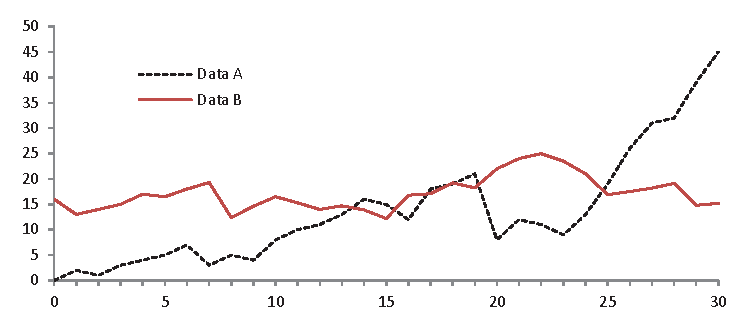
\includegraphics[width=\textwidth]{fig1.eps}
\caption{A figure caption is always placed below the illustration.
Please note that short captions are centered, while long ones are
justified by the macro package automatically.} \label{fig1}
\end{figure}

\begin{theorem}
This is a sample theorem. The run-in heading is set in bold, while
the following text appears in italics. Definitions, lemmas,
propositions, and corollaries are styled the same way.
\end{theorem}
%
% the environments 'definition', 'lemma', 'proposition', 'corollary',
% 'remark', and 'example' are defined in the LLNCS documentclass as well.
%
\begin{proof}
Proofs, examples, and remarks have the initial word in italics,
while the following text appears in normal font.
\end{proof}
For citations of references, we prefer the use of square brackets
and consecutive numbers. Citations using labels or the author/year
convention are also acceptable. The following bibliography provides
a sample reference list with entries for journal
articles~\cite{ref_article1}, an LNCS chapter~\cite{ref_lncs1}, a
book~\cite{ref_book1}, proceedings without editors~\cite{ref_proc1},
and a homepage~\cite{ref_url1}. Multiple citations are grouped
\cite{ref_article1,ref_lncs1,ref_book1},
\cite{ref_article1,ref_book1,ref_proc1,ref_url1}.
%
% ---- Bibliography ----
%
% BibTeX users should specify bibliography style 'splncs04'.
% References will then be sorted and formatted in the correct style.
%
% \bibliographystyle{splncs04}
% \bibliography{mybibliography}
%
\begin{thebibliography}{8}
\bibitem{ref_article1}
Author, F.: Article title. Journal \textbf{2}(5), 99--110 (2016)

\bibitem{ref_lncs1}
Author, F., Author, S.: Title of a proceedings paper. In: Editor,
F., Editor, S. (eds.) CONFERENCE 2016, LNCS, vol. 9999, pp. 1--13.
Springer, Heidelberg (2016). \doi{10.10007/1234567890}

\bibitem{ref_book1}
Author, F., Author, S., Author, T.: Book title. 2nd edn. Publisher,
Location (1999)

\bibitem{ref_proc1}
Author, A.-B.: Contribution title. In: 9th International Proceedings
on Proceedings, pp. 1--2. Publisher, Location (2010)

\bibitem{ref_url1}
LNCS Homepage, \url{http://www.springer.com/lncs}. Last accessed 4
Oct 2017
\end{thebibliography}
\end{document}
